\documentclass[border=10pt]{standalone}
\usepackage[european]{circuitikz}
\begin{document}
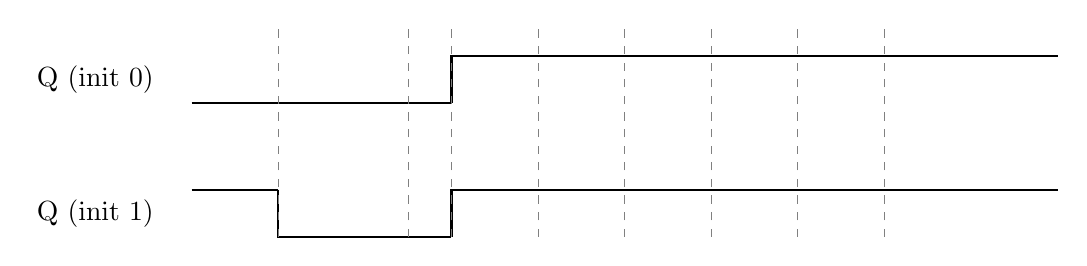
\begin{tikzpicture}[x=1cm, y=1cm, font=\normalsize, line width=0.8pt]
  % 8.2 答案波形：两行 Q（上=初态0、下=初态1），横轴 0–100% 20 格，每格 0.55cm。
  %   CP 四脉冲 10–25/30–40/50–60/70–80%（与 fig-8-02-3row 同刻度）。
  %   初态 0：0–30% 低，30% 处置 1，此后恒 1。
  %   初态 1：0–10% 高，10%(CP₁↑)置 0，30%(CP₂↑)置 1，此后恒 1。
  %   两行自 30% 起重合。竖虚线在 10/25/30/40/50/60/70/80% 八处。
  \def\seg{0.55}
  \def\hi{0.6}
  \def\total{11.0}

  % 上：初态 0
  \begin{scope}[yshift=0cm]
    \node[anchor=east] at (-0.35,\hi/2) {Q (init 0)};
    \draw (0,0) -- (6*\seg,0);
    \draw (6*\seg,0) -- (6*\seg,\hi) -- (\total,\hi);
  \end{scope}

  % 下：初态 1
  \begin{scope}[yshift=-1.7cm]
    \node[anchor=east] at (-0.35,\hi/2) {Q (init 1)};
    \draw (0,\hi) -- (2*\seg,\hi);
    \draw (2*\seg,\hi) -- (2*\seg,0) -- (6*\seg,0);
    \draw (6*\seg,0) -- (6*\seg,\hi) -- (\total,\hi);
  \end{scope}

  % 八条竖虚线（贯穿两行，不压字）
  \foreach \g in {2,5,6,8,10,12,14,16} {
    \draw[dashed, gray, line width=0.4pt] (\g*\seg,-1.7) -- (\g*\seg,0.95);
  }

\end{tikzpicture}
\end{document}
